%%%%%%%%%%%%%%%%%%%%%%%%%%%%%%%%%%%%%%%%%%%%%%%%%%%%%%%%%%%%
% 6.1 DISCRETE STRUCTURES
% The Composition of Advanced Mathematics
%%%%%%%%%%%%%%%%%%%%%%%%%%%%%%%%%%%%%%%%%%%%%%%%%%%%%%%%%%%%

\section{Discrete Structures}
\label{sec:discrete-structures}

\prerequisite{
Sets, functions, relations, elementary logic, basic algebraic notation,
and familiarity with finite mathematical objects.
}

\learningobjectives{
By the end of this section, the reader should be able to:
\begin{itemize}
    \item explain what distinguishes a discrete mathematical structure
          from a continuous one;
    \item describe finite and countably infinite collections;
    \item work with tuples, Cartesian products, strings, sequences,
          multisets, and families of sets;
    \item represent subsets using indicator functions and binary vectors;
    \item interpret relations as subsets of Cartesian products;
    \item recognize equivalence relations and partitions;
    \item recognize partial orders and ordered structures;
    \item describe incidence structures and hypergraphs;
    \item understand recursive and inductively defined structures;
    \item distinguish labeled from unlabeled objects;
    \item explain structural equivalence through isomorphism;
    \item identify invariants of discrete structures;
    \item recognize combinatorial classes graded by size;
    \item understand how discrete objects are encoded for computation;
    \item connect discrete structures with counting, graph theory,
          combinatorics, probability, algorithms, and optimization.
\end{itemize}
}

%%%%%%%%%%%%%%%%%%%%%%%%%%%%%%%%%%%%%%%%%%%%%%%%%%%%%%%%%%%%
\subsection{What Is a Discrete Structure?}
\label{subsec:what-is-discrete-structure}
%%%%%%%%%%%%%%%%%%%%%%%%%%%%%%%%%%%%%%%%%%%%%%%%%%%%%%%%%%%%

A large portion of mathematics studies objects that vary continuously.

For example, a real-valued variable may range over an interval such as

\[
[0,1].
\]

Between two distinct real numbers there are infinitely many additional
real numbers.

Discrete mathematics instead focuses primarily on objects built from
separate, distinguishable pieces.

Typical examples include:

\begin{itemize}
    \item integers;
    \item finite sets;
    \item strings;
    \item permutations;
    \item graphs;
    \item trees;
    \item partitions;
    \item finite sequences;
    \item logical assignments;
    \item networks;
    \item schedules;
    \item arrangements;
    \item combinatorial designs.
\end{itemize}

\begin{definitionbox}{Discrete Structure}
A \emph{discrete structure} is a mathematical object whose relevant
components are distinguishable as separate units and are usually
organized through finite or countably infinite relationships.
\end{definitionbox}

The word \emph{discrete} comes from the idea of separation.

The central contrast is

\[
\boxed{
\text{discrete}
\qquad\text{versus}\qquad
\text{continuous}.
}
\]

This distinction is conceptual rather than absolute. A problem may
contain both discrete and continuous components.

%%%%%%%%%%%%%%%%%%%%%%%%%%%%%%%%%%%%%%%%%%%%%%%%%%%%%%%%%%%%
\subsection{Discrete Versus Continuous Models}
\label{subsec:discrete-versus-continuous}
%%%%%%%%%%%%%%%%%%%%%%%%%%%%%%%%%%%%%%%%%%%%%%%%%%%%%%%%%%%%

Consider the possible number of students in a classroom.

The quantity may take values

\[
0,1,2,3,\ldots
\]

but not

\[
2.4
\]

students.

This is naturally modeled discretely.

By contrast, the temperature of the classroom may be modeled by a real
variable

\[
T\in\mathbb{R}.
\]

The first variable is integer-valued, while the second is commonly
treated as continuous.

\begin{conceptbox}
A discrete model usually describes \emph{which objects exist}, how many
there are, how they are arranged, or how they are related.

A continuous model usually describes quantities that vary over an
interval or geometric region.
\end{conceptbox}

Many applied problems combine both.

For example, an airline scheduling problem may contain:

\[
\text{discrete decisions}
+
\text{continuous times and costs}.
\]

%%%%%%%%%%%%%%%%%%%%%%%%%%%%%%%%%%%%%%%%%%%%%%%%%%%%%%%%%%%%
\subsection{Finite and Infinite Discrete Sets}
\label{subsec:finite-infinite-discrete}
%%%%%%%%%%%%%%%%%%%%%%%%%%%%%%%%%%%%%%%%%%%%%%%%%%%%%%%%%%%%

The simplest discrete structures are finite sets.

For example,

\[
A=\{a,b,c,d\}
\]

has cardinality

\[
|A|=4.
\]

The vertical-bar notation

\[
|A|
\]

is read ``the cardinality of \(A\)'' or ``the size of \(A\).''

Discrete structures need not be finite.

The integers

\[
\mathbb{Z}
=
\{\ldots,-2,-1,0,1,2,\ldots\}
\]

form an infinite discrete set.

Similarly,

\[
\mathbb{N}
=
\{0,1,2,3,\ldots\}
\]

is countably infinite under the convention used here.

\begin{importantbox}
Discrete does not mean finite.

A structure may be infinite while still being discrete.
\end{importantbox}

%%%%%%%%%%%%%%%%%%%%%%%%%%%%%%%%%%%%%%%%%%%%%%%%%%%%%%%%%%%%
\subsection{Countability}
\label{subsec:discrete-countability}
%%%%%%%%%%%%%%%%%%%%%%%%%%%%%%%%%%%%%%%%%%%%%%%%%%%%%%%%%%%%

A set is countably infinite when its elements can be placed in
one-to-one correspondence with the natural numbers.

Thus a countably infinite set may be listed as

\[
a_0,a_1,a_2,a_3,\ldots.
\]

Examples include:

\[
\mathbb{N},
\qquad
\mathbb{Z},
\qquad
\mathbb{Q}.
\]

The rational numbers are dense in the real numbers, yet they are
countable.

The real numbers

\[
\mathbb{R}
\]

are uncountable.

The distinction between finite, countably infinite, and uncountable
sets was developed more generally in the foundational material of this
text.

For combinatorics, most of our primary objects will be finite, although
infinite discrete structures will appear throughout the subject.

%%%%%%%%%%%%%%%%%%%%%%%%%%%%%%%%%%%%%%%%%%%%%%%%%%%%%%%%%%%%
\subsection{Tuples}
\label{subsec:discrete-tuples}
%%%%%%%%%%%%%%%%%%%%%%%%%%%%%%%%%%%%%%%%%%%%%%%%%%%%%%%%%%%%

An ordered collection of objects is called a tuple.

For example,

\[
(a,b,c)
\]

is an ordered triple.

Unlike a set,

\[
(a,b,c)
\neq
(c,b,a)
\]

in general.

A general \(n\)-tuple has the form

\[
\boxed{
(a_1,a_2,\ldots,a_n).
}
\]

The integer \(n\) records the length of the tuple.

Tuples are fundamental because many discrete objects can be encoded as
ordered collections.

%%%%%%%%%%%%%%%%%%%%%%%%%%%%%%%%%%%%%%%%%%%%%%%%%%%%%%%%%%%%
\subsection{Cartesian Products}
\label{subsec:discrete-cartesian-products}
%%%%%%%%%%%%%%%%%%%%%%%%%%%%%%%%%%%%%%%%%%%%%%%%%%%%%%%%%%%%

Given sets \(A\) and \(B\), their Cartesian product is

\[
\boxed{
A\times B
=
\{(a,b):a\in A,\ b\in B\}.
}
\]

The symbol

\[
\times
\]

is read ``cross'' in this context.

If

\[
|A|=m
\]

and

\[
|B|=n,
\]

then

\[
\boxed{
|A\times B|=mn.
}
\]

This basic fact will later become one of the first counting principles.

More generally,

\[
A_1\times A_2\times\cdots\times A_n
\]

contains all tuples

\[
(a_1,a_2,\ldots,a_n)
\]

with

\[
a_i\in A_i.
\]

If all sets are finite, then

\[
\boxed{
\left|
A_1\times\cdots\times A_n
\right|
=
\prod_{i=1}^{n}|A_i|.
}
\]

%%%%%%%%%%%%%%%%%%%%%%%%%%%%%%%%%%%%%%%%%%%%%%%%%%%%%%%%%%%%
\subsection{Worked Example: Cartesian Product}
\label{subsec:worked-cartesian-product}
%%%%%%%%%%%%%%%%%%%%%%%%%%%%%%%%%%%%%%%%%%%%%%%%%%%%%%%%%%%%

\begin{workedexamplebox}{Forming Ordered Pairs}

Let

\[
A=\{1,2\}
\]

and

\[
B=\{x,y,z\}.
\]

Then

\[
A\times B
=
\{
(1,x),(1,y),(1,z),
(2,x),(2,y),(2,z)
\}.
\]

Since

\[
|A|=2
\]

and

\[
|B|=3,
\]

we have

\[
|A\times B|=2\cdot3.
\]

\begin{answerbox}
\[
\boxed{
|A\times B|=6.
}
\]
\end{answerbox}

\end{workedexamplebox}

%%%%%%%%%%%%%%%%%%%%%%%%%%%%%%%%%%%%%%%%%%%%%%%%%%%%%%%%%%%%
\subsection{Sequences}
\label{subsec:discrete-sequences}
%%%%%%%%%%%%%%%%%%%%%%%%%%%%%%%%%%%%%%%%%%%%%%%%%%%%%%%%%%%%

A sequence is an ordered list indexed by integers.

A finite sequence may be written

\[
\boxed{
a_1,a_2,\ldots,a_n.
}
\]

An infinite sequence may be written

\[
\boxed{
(a_n)_{n\geq0}.
}
\]

The notation

\[
(a_n)_{n\geq0}
\]

is read ``the sequence \(a_n\) for \(n\) greater than or equal to
zero.''

Formally, a sequence may be interpreted as a function whose domain is
an index set such as

\[
\{1,\ldots,n\}
\]

or

\[
\mathbb{N}.
\]

Thus sequences connect the language of functions with ordered discrete
data.

%%%%%%%%%%%%%%%%%%%%%%%%%%%%%%%%%%%%%%%%%%%%%%%%%%%%%%%%%%%%
\subsection{Strings and Alphabets}
\label{subsec:strings-alphabets}
%%%%%%%%%%%%%%%%%%%%%%%%%%%%%%%%%%%%%%%%%%%%%%%%%%%%%%%%%%%%

Many discrete structures arise from finite strings.

\begin{definitionbox}{Alphabet}
An \emph{alphabet} is a finite set of symbols.
\end{definitionbox}

An alphabet is often denoted

\[
\Sigma.
\]

The Greek capital letter

\[
\Sigma
\]

is called ``capital sigma.''

For example,

\[
\Sigma=\{0,1\}
\]

is the binary alphabet.

A string of length \(n\) over \(\Sigma\) is an ordered sequence

\[
\boxed{
a_1a_2\cdots a_n,
\qquad
a_i\in\Sigma.
}
\]

The set of all strings of length \(n\) is denoted

\[
\boxed{
\Sigma^n.
}
\]

If

\[
|\Sigma|=k,
\]

then

\[
\boxed{
|\Sigma^n|=k^n.
}
\]

%%%%%%%%%%%%%%%%%%%%%%%%%%%%%%%%%%%%%%%%%%%%%%%%%%%%%%%%%%%%
\subsection{The Empty String}
\label{subsec:empty-string}
%%%%%%%%%%%%%%%%%%%%%%%%%%%%%%%%%%%%%%%%%%%%%%%%%%%%%%%%%%%%

There is exactly one string of length zero.

It is called the empty string and is commonly denoted

\[
\boxed{
\varepsilon.
}
\]

The Greek letter

\[
\varepsilon
\]

is called ``epsilon.''

Thus

\[
|\varepsilon|=0.
\]

The empty string plays a role analogous to the empty set in set theory.

%%%%%%%%%%%%%%%%%%%%%%%%%%%%%%%%%%%%%%%%%%%%%%%%%%%%%%%%%%%%
\subsection{All Finite Strings}
\label{subsec:all-finite-strings}
%%%%%%%%%%%%%%%%%%%%%%%%%%%%%%%%%%%%%%%%%%%%%%%%%%%%%%%%%%%%

The set of all finite strings over an alphabet \(\Sigma\) is denoted

\[
\boxed{
\Sigma^{*}.
}
\]

The star is called the \emph{Kleene star} in theoretical computer
science.

It represents

\[
\boxed{
\Sigma^{*}
=
\bigcup_{n=0}^{\infty}\Sigma^n.
}
\]

Thus

\[
\varepsilon\in\Sigma^{*}.
\]

A language over \(\Sigma\) is any subset

\[
L\subseteq\Sigma^{*}.
\]

This simple construction becomes important in automata theory,
computability, coding theory, and formal languages.

%%%%%%%%%%%%%%%%%%%%%%%%%%%%%%%%%%%%%%%%%%%%%%%%%%%%%%%%%%%%
\subsection{Binary Strings}
\label{subsec:binary-strings}
%%%%%%%%%%%%%%%%%%%%%%%%%%%%%%%%%%%%%%%%%%%%%%%%%%%%%%%%%%%%

A binary string uses the alphabet

\[
\{0,1\}.
\]

For example,

\[
1011001
\]

is a binary string of length \(7\).

The collection of binary strings of length \(n\) is

\[
\boxed{
\{0,1\}^n.
}
\]

Its cardinality is

\[
\boxed{
2^n.
}
\]

Binary strings appear throughout discrete mathematics because a binary
choice naturally represents a yes-or-no decision.

%%%%%%%%%%%%%%%%%%%%%%%%%%%%%%%%%%%%%%%%%%%%%%%%%%%%%%%%%%%%
\subsection{Bit Vectors}
\label{subsec:bit-vectors}
%%%%%%%%%%%%%%%%%%%%%%%%%%%%%%%%%%%%%%%%%%%%%%%%%%%%%%%%%%%%

A binary string may also be regarded as a vector

\[
\boxed{
x=(x_1,\ldots,x_n),
\qquad
x_i\in\{0,1\}.
}
\]

Such an object is often called a \emph{bit vector} or \emph{binary
vector}.

For example,

\[
x=(1,0,1,1,0)
\]

has five coordinates.

Bit vectors provide a useful bridge between set theory, Boolean
algebra, coding theory, probability, and discrete optimization.

%%%%%%%%%%%%%%%%%%%%%%%%%%%%%%%%%%%%%%%%%%%%%%%%%%%%%%%%%%%%
\subsection{Subsets as Binary Vectors}
\label{subsec:subsets-binary-vectors}
%%%%%%%%%%%%%%%%%%%%%%%%%%%%%%%%%%%%%%%%%%%%%%%%%%%%%%%%%%%%

Let

\[
S=\{s_1,s_2,\ldots,s_n\}.
\]

Every subset

\[
A\subseteq S
\]

can be represented by a binary vector

\[
(x_1,\ldots,x_n),
\]

where

\[
x_i=
\begin{cases}
1,&s_i\in A,\\
0,&s_i\notin A.
\end{cases}
\]

Thus subsets of an \(n\)-element set correspond exactly to binary
strings of length \(n\).

Therefore,

\[
\boxed{
|\mathcal{P}(S)|=2^n,
}
\]

where

\[
\mathcal{P}(S)
\]

denotes the power set of \(S\).

This representation will be used repeatedly in combinatorics.

%%%%%%%%%%%%%%%%%%%%%%%%%%%%%%%%%%%%%%%%%%%%%%%%%%%%%%%%%%%%
\subsection{Indicator Functions}
\label{subsec:indicator-functions}
%%%%%%%%%%%%%%%%%%%%%%%%%%%%%%%%%%%%%%%%%%%%%%%%%%%%%%%%%%%%

The binary representation of a subset can be expressed using an
indicator function.

\begin{definitionbox}{Indicator Function}
For \(A\subseteq S\), the indicator function of \(A\) is

\[
\boxed{
\mathbf{1}_A(x)
=
\begin{cases}
1,&x\in A,\\
0,&x\notin A.
\end{cases}
}
\]
\end{definitionbox}

The symbol

\[
\mathbf{1}_A
\]

is read ``the indicator of \(A\).''

Some authors use

\[
\chi_A
\]

instead.

The Greek letter

\[
\chi
\]

is called ``chi.''

Indicator functions convert set membership into arithmetic.

For example,

\[
|A|
=
\sum_{x\in S}\mathbf{1}_A(x).
\]

%%%%%%%%%%%%%%%%%%%%%%%%%%%%%%%%%%%%%%%%%%%%%%%%%%%%%%%%%%%%
\subsection{Set Operations with Indicators}
\label{subsec:set-operations-indicators}
%%%%%%%%%%%%%%%%%%%%%%%%%%%%%%%%%%%%%%%%%%%%%%%%%%%%%%%%%%%%

Indicator functions allow familiar set operations to be expressed
algebraically.

For example,

\[
\boxed{
\mathbf{1}_{A\cap B}(x)
=
\mathbf{1}_A(x)\mathbf{1}_B(x).
}
\]

Also,

\[
\boxed{
\mathbf{1}_{A^c}(x)
=
1-\mathbf{1}_A(x),
}
\]

where the complement is taken relative to a fixed universe.

For unions,

\[
\boxed{
\mathbf{1}_{A\cup B}(x)
=
\mathbf{1}_A(x)
+
\mathbf{1}_B(x)
-
\mathbf{1}_A(x)\mathbf{1}_B(x).
}
\]

These identities are useful in probability and combinatorics.

%%%%%%%%%%%%%%%%%%%%%%%%%%%%%%%%%%%%%%%%%%%%%%%%%%%%%%%%%%%%
\subsection{Hamming Weight}
\label{subsec:hamming-weight}
%%%%%%%%%%%%%%%%%%%%%%%%%%%%%%%%%%%%%%%%%%%%%%%%%%%%%%%%%%%%

For a binary vector

\[
x=(x_1,\ldots,x_n),
\]

the number of coordinates equal to \(1\) is called its Hamming weight.

It is written

\[
\boxed{
\operatorname{wt}(x)
=
\sum_{i=1}^{n}x_i.
}
\]

For example,

\[
x=(1,0,1,1,0,1)
\]

has

\[
\operatorname{wt}(x)=4.
\]

If \(x\) represents a subset \(A\), then

\[
\boxed{
\operatorname{wt}(x)=|A|.
}
\]

%%%%%%%%%%%%%%%%%%%%%%%%%%%%%%%%%%%%%%%%%%%%%%%%%%%%%%%%%%%%
\subsection{Hamming Distance}
\label{subsec:hamming-distance}
%%%%%%%%%%%%%%%%%%%%%%%%%%%%%%%%%%%%%%%%%%%%%%%%%%%%%%%%%%%%

For two binary strings \(x\) and \(y\) of equal length, the Hamming
distance

\[
d_H(x,y)
\]

is the number of coordinates in which they differ.

For example,

\[
x=101101,
\qquad
y=111001.
\]

They differ in two positions, so

\[
\boxed{
d_H(x,y)=2.
}
\]

The subscript \(H\) refers to Richard Hamming.

Hamming distance is fundamental in coding theory, information theory,
Boolean analysis, and computational biology.

%%%%%%%%%%%%%%%%%%%%%%%%%%%%%%%%%%%%%%%%%%%%%%%%%%%%%%%%%%%%
\subsection{Families of Sets}
\label{subsec:families-of-sets}
%%%%%%%%%%%%%%%%%%%%%%%%%%%%%%%%%%%%%%%%%%%%%%%%%%%%%%%%%%%%

A collection whose elements are themselves sets is often called a
\emph{family of sets}.

For example,

\[
\mathcal{F}
=
\{
\{1,2\},
\{1,3\},
\{2,3\}
\}.
\]

The calligraphic letter

\[
\mathcal{F}
\]

is read ``calligraphic F.''

Set families are central objects in combinatorics.

A common example is the family of all \(k\)-element subsets of an
\(n\)-element set.

%%%%%%%%%%%%%%%%%%%%%%%%%%%%%%%%%%%%%%%%%%%%%%%%%%%%%%%%%%%%
\subsection{The Set of \(k\)-Subsets}
\label{subsec:k-subsets}
%%%%%%%%%%%%%%%%%%%%%%%%%%%%%%%%%%%%%%%%%%%%%%%%%%%%%%%%%%%%

If \(S\) is a finite set, the notation

\[
\boxed{
\binom{S}{k}
}
\]

may be used for the family of all \(k\)-element subsets of \(S\).

Thus

\[
\binom{S}{k}
=
\{A\subseteq S:|A|=k\}.
\]

When

\[
|S|=n,
\]

the number of such subsets is

\[
\boxed{
\left|\binom{S}{k}\right|
=
\binom{n}{k}.
}
\]

The numerical quantity

\[
\binom{n}{k}
\]

will be studied systematically in the next section.

%%%%%%%%%%%%%%%%%%%%%%%%%%%%%%%%%%%%%%%%%%%%%%%%%%%%%%%%%%%%
\subsection{Multisets}
\label{subsec:multisets}
%%%%%%%%%%%%%%%%%%%%%%%%%%%%%%%%%%%%%%%%%%%%%%%%%%%%%%%%%%%%

Ordinary sets do not record repeated elements.

A multiset does.

For example,

\[
\{a,a,a,b,b,c\}
\]

contains:

\[
3\text{ copies of }a,
\qquad
2\text{ copies of }b,
\qquad
1\text{ copy of }c.
\]

\begin{definitionbox}{Multiset}
A \emph{multiset} is a collection in which an element may occur with a
specified nonnegative integer multiplicity.
\end{definitionbox}

If the underlying universe is

\[
S=\{s_1,\ldots,s_n\},
\]

a finite multiset may be represented by a multiplicity vector

\[
\boxed{
(m_1,\ldots,m_n),
\qquad
m_i\in\mathbb{Z}_{\geq0}.
}
\]

%%%%%%%%%%%%%%%%%%%%%%%%%%%%%%%%%%%%%%%%%%%%%%%%%%%%%%%%%%%%
\subsection{Multiplicity}
\label{subsec:multiplicity}
%%%%%%%%%%%%%%%%%%%%%%%%%%%%%%%%%%%%%%%%%%%%%%%%%%%%%%%%%%%%

The multiplicity of an element \(x\) in a multiset \(M\) records how
many times \(x\) appears.

It may be written

\[
m_M(x).
\]

For example, if

\[
M=\{a,a,a,b,b,c\},
\]

then

\[
m_M(a)=3,
\qquad
m_M(b)=2,
\qquad
m_M(c)=1.
\]

The total size of the multiset is

\[
\boxed{
|M|
=
\sum_x m_M(x).
}
\]

%%%%%%%%%%%%%%%%%%%%%%%%%%%%%%%%%%%%%%%%%%%%%%%%%%%%%%%%%%%%
\subsection{Relations}
\label{subsec:discrete-relations}
%%%%%%%%%%%%%%%%%%%%%%%%%%%%%%%%%%%%%%%%%%%%%%%%%%%%%%%%%%%%

Relations organize connections among discrete objects.

\begin{definitionbox}{Binary Relation}
A binary relation from a set \(A\) to a set \(B\) is a subset

\[
\boxed{
R\subseteq A\times B.
}
\]
\end{definitionbox}

If

\[
(a,b)\in R,
\]

we may write

\[
\boxed{
aRb.
}
\]

A relation on \(A\) is a subset

\[
R\subseteq A\times A.
\]

%%%%%%%%%%%%%%%%%%%%%%%%%%%%%%%%%%%%%%%%%%%%%%%%%%%%%%%%%%%%
\subsection{Relations as Tables}
\label{subsec:relations-tables}
%%%%%%%%%%%%%%%%%%%%%%%%%%%%%%%%%%%%%%%%%%%%%%%%%%%%%%%%%%%%

Suppose

\[
A=\{1,2,3\}
\]

and define

\[
R=\{(1,2),(1,3),(2,3)\}.
\]

The relation may be represented by a \(0\)-\(1\) matrix

\[
M_R
=
\begin{pmatrix}
0&1&1\\
0&0&1\\
0&0&0
\end{pmatrix}.
\]

The entry in row \(i\), column \(j\) equals \(1\) exactly when

\[
iRj.
\]

This matrix representation will later become especially important in
graph theory.

%%%%%%%%%%%%%%%%%%%%%%%%%%%%%%%%%%%%%%%%%%%%%%%%%%%%%%%%%%%%
\subsection{Relations as Directed Connections}
\label{subsec:relations-directed}
%%%%%%%%%%%%%%%%%%%%%%%%%%%%%%%%%%%%%%%%%%%%%%%%%%%%%%%%%%%%

A relation on a finite set may also be visualized using directed
arrows.

If

\[
aRb,
\]

draw an arrow

\[
a\longrightarrow b.
\]

Thus a finite binary relation can naturally be regarded as a directed
network.

This observation leads directly toward directed graphs.

%%%%%%%%%%%%%%%%%%%%%%%%%%%%%%%%%%%%%%%%%%%%%%%%%%%%%%%%%%%%
\subsection{Properties of Relations}
\label{subsec:properties-relations-review}
%%%%%%%%%%%%%%%%%%%%%%%%%%%%%%%%%%%%%%%%%%%%%%%%%%%%%%%%%%%%

Several properties of relations recur throughout discrete mathematics.

A relation \(R\) on \(A\) is:

\begin{itemize}
    \item \textbf{reflexive} if
    \[
    aRa
    \]
    for every \(a\in A\);

    \item \textbf{symmetric} if
    \[
    aRb\Longrightarrow bRa;
    \]

    \item \textbf{antisymmetric} if
    \[
    aRb\text{ and }bRa
    \Longrightarrow
    a=b;
    \]

    \item \textbf{transitive} if
    \[
    aRb\text{ and }bRc
    \Longrightarrow
    aRc.
    \]
\end{itemize}

These concepts were introduced earlier in the foundational chapters and
are recalled here because they generate important discrete structures.

%%%%%%%%%%%%%%%%%%%%%%%%%%%%%%%%%%%%%%%%%%%%%%%%%%%%%%%%%%%%
\subsection{Equivalence Relations}
\label{subsec:equivalence-relations-discrete}
%%%%%%%%%%%%%%%%%%%%%%%%%%%%%%%%%%%%%%%%%%%%%%%%%%%%%%%%%%%%

A relation is an equivalence relation if it is:

\[
\boxed{
\text{reflexive}
+
\text{symmetric}
+
\text{transitive}.
}
\]

If \(R\) is an equivalence relation on \(A\), then the equivalence class
of \(a\) is

\[
\boxed{
[a]
=
\{x\in A:xRa\}.
}
\]

Equivalence relations organize objects according to when they should be
considered ``the same'' for a particular purpose.

%%%%%%%%%%%%%%%%%%%%%%%%%%%%%%%%%%%%%%%%%%%%%%%%%%%%%%%%%%%%
\subsection{Partitions}
\label{subsec:partitions-discrete}
%%%%%%%%%%%%%%%%%%%%%%%%%%%%%%%%%%%%%%%%%%%%%%%%%%%%%%%%%%%%

\begin{definitionbox}{Partition}
A partition of a set \(A\) is a collection of nonempty subsets

\[
A_1,A_2,\ldots,A_k
\]

such that

\[
A_i\cap A_j=\varnothing
\qquad
(i\neq j)
\]

and

\[
\boxed{
A_1\cup A_2\cup\cdots\cup A_k=A.
}
\]
\end{definitionbox}

The sets \(A_i\) are called the \emph{blocks} of the partition.

Equivalence relations and partitions describe the same underlying
structure.

Every equivalence relation determines a partition into equivalence
classes, and every partition determines an equivalence relation.

%%%%%%%%%%%%%%%%%%%%%%%%%%%%%%%%%%%%%%%%%%%%%%%%%%%%%%%%%%%%
\subsection{Worked Example: Partition}
\label{subsec:worked-partition}
%%%%%%%%%%%%%%%%%%%%%%%%%%%%%%%%%%%%%%%%%%%%%%%%%%%%%%%%%%%%

\begin{workedexamplebox}{Congruence Classes Modulo \(3\)}

Consider the integers

\[
\mathbb{Z}.
\]

Define

\[
a\sim b
\]

when

\[
a\equiv b\pmod 3.
\]

The equivalence classes are

\[
[0],
\qquad
[1],
\qquad
[2].
\]

They consist of integers having the same remainder after division by
\(3\).

\begin{answerbox}
The integers are partitioned as

\[
\boxed{
\mathbb{Z}
=
[0]\cup[1]\cup[2],
}
\]

where the three classes are pairwise disjoint.
\end{answerbox}

\end{workedexamplebox}

%%%%%%%%%%%%%%%%%%%%%%%%%%%%%%%%%%%%%%%%%%%%%%%%%%%%%%%%%%%%
\subsection{Partial Orders}
\label{subsec:partial-orders-discrete}
%%%%%%%%%%%%%%%%%%%%%%%%%%%%%%%%%%%%%%%%%%%%%%%%%%%%%%%%%%%%

A relation \(\preceq\) on a set \(P\) is a partial order when it is:

\[
\boxed{
\text{reflexive}
+
\text{antisymmetric}
+
\text{transitive}.
}
\]

The pair

\[
(P,\preceq)
\]

is called a partially ordered set, or \emph{poset}.

The symbol

\[
\preceq
\]

is read ``precedes or equals'' or, depending on context, ``is less than
or equal to in the order.''

Examples include:

\[
(\mathcal{P}(S),\subseteq)
\]

and divisibility on positive integers.

A more advanced treatment of ordered algebraic structures and lattices
appears in Chapter~\ref{chap:algebra}.

%%%%%%%%%%%%%%%%%%%%%%%%%%%%%%%%%%%%%%%%%%%%%%%%%%%%%%%%%%%%
\subsection{Comparability}
\label{subsec:comparability}
%%%%%%%%%%%%%%%%%%%%%%%%%%%%%%%%%%%%%%%%%%%%%%%%%%%%%%%%%%%%

Two elements \(x,y\in P\) are comparable when

\[
x\preceq y
\]

or

\[
y\preceq x.
\]

Otherwise they are incomparable.

A partial order does not require every pair to be comparable.

If every pair is comparable, the order is called a \emph{total order}
or \emph{linear order}.

Thus,

\[
\boxed{
\text{total order}
\Longrightarrow
\text{partial order}.
}
\]

The converse is false.

%%%%%%%%%%%%%%%%%%%%%%%%%%%%%%%%%%%%%%%%%%%%%%%%%%%%%%%%%%%%
\subsection{Hasse Diagrams}
\label{subsec:hasse-diagrams-discrete}
%%%%%%%%%%%%%%%%%%%%%%%%%%%%%%%%%%%%%%%%%%%%%%%%%%%%%%%%%%%%

Finite partial orders are often represented by Hasse diagrams.

In a Hasse diagram:

\begin{itemize}
    \item elements are represented by points;
    \item larger elements are drawn above smaller elements;
    \item transitive edges are omitted;
    \item loops from reflexivity are omitted.
\end{itemize}

For the power set

\[
\mathcal{P}(\{1,2\})
\]

ordered by inclusion, the structure is

\begin{centereddiagram}
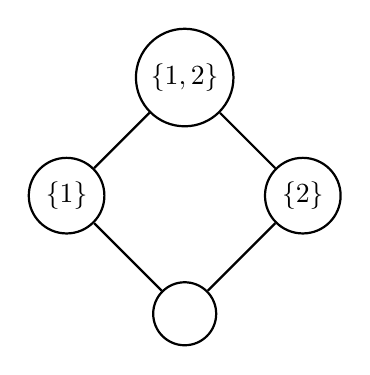
\begin{tikzpicture}[
    every node/.style={circle,draw,minimum size=8mm},
    line width=0.8pt
]
\node (empty) at (0,0) {$\varnothing$};
\node (one) at (-1.5,1.5) {$\{1\}$};
\node (two) at (1.5,1.5) {$\{2\}$};
\node (both) at (0,3) {$\{1,2\}$};

\draw (empty)--(one);
\draw (empty)--(two);
\draw (one)--(both);
\draw (two)--(both);
\end{tikzpicture}
\end{centereddiagram}

This diagram records the inclusion structure.

%%%%%%%%%%%%%%%%%%%%%%%%%%%%%%%%%%%%%%%%%%%%%%%%%%%%%%%%%%%%
\subsection{Chains and Antichains}
\label{subsec:chains-antichains-discrete}
%%%%%%%%%%%%%%%%%%%%%%%%%%%%%%%%%%%%%%%%%%%%%%%%%%%%%%%%%%%%

A subset \(C\subseteq P\) is a \emph{chain} if every pair of elements
in \(C\) is comparable.

A subset \(A\subseteq P\) is an \emph{antichain} if no two distinct
elements in \(A\) are comparable.

For example, in

\[
\mathcal{P}(\{1,2,3\})
\]

ordered by inclusion,

\[
\varnothing
\subset
\{1\}
\subset
\{1,2\}
\subset
\{1,2,3\}
\]

forms a chain.

Meanwhile,

\[
\{1\},
\qquad
\{2\},
\qquad
\{3\}
\]

forms an antichain.

Chains and antichains later play major roles in extremal combinatorics.

%%%%%%%%%%%%%%%%%%%%%%%%%%%%%%%%%%%%%%%%%%%%%%%%%%%%%%%%%%%%
\subsection{Directed and Undirected Structures}
\label{subsec:directed-undirected-structures}
%%%%%%%%%%%%%%%%%%%%%%%%%%%%%%%%%%%%%%%%%%%%%%%%%%%%%%%%%%%%

A relation distinguishes ordered pairs

\[
(a,b)
\]

from

\[
(b,a).
\]

Some discrete relationships are directional.

Examples include:

\[
\text{``is a prerequisite for''}
\]

and

\[
\text{``sends information to.''}
\]

Other relationships are naturally symmetric.

Examples include:

\[
\text{``is connected to''}
\]

and

\[
\text{``is adjacent to.''}
\]

This distinction motivates directed and undirected graph structures,
which will be studied systematically later in this chapter.

%%%%%%%%%%%%%%%%%%%%%%%%%%%%%%%%%%%%%%%%%%%%%%%%%%%%%%%%%%%%
\subsection{Incidence Structures}
\label{subsec:incidence-structures}
%%%%%%%%%%%%%%%%%%%%%%%%%%%%%%%%%%%%%%%%%%%%%%%%%%%%%%%%%%%%

A broad class of discrete structures records which objects are incident
with which other objects.

Suppose \(P\) is a set of points and \(B\) is a family of blocks.

An incidence relation

\[
I\subseteq P\times B
\]

specifies when a point lies in a block.

We may write

\[
pIb
\]

to mean that point \(p\) is incident with block \(b\).

Incidence structures provide a common framework for:

\begin{itemize}
    \item finite geometries;
    \item block designs;
    \item hypergraphs;
    \item networks;
    \item experimental designs.
\end{itemize}

%%%%%%%%%%%%%%%%%%%%%%%%%%%%%%%%%%%%%%%%%%%%%%%%%%%%%%%%%%%%
\subsection{Incidence Matrices}
\label{subsec:incidence-matrices-discrete}
%%%%%%%%%%%%%%%%%%%%%%%%%%%%%%%%%%%%%%%%%%%%%%%%%%%%%%%%%%%%

If

\[
P=\{p_1,\ldots,p_v\}
\]

and

\[
B=\{B_1,\ldots,B_b\},
\]

the incidence matrix is the \(v\times b\) matrix

\[
M=(m_{ij}),
\]

where

\[
\boxed{
m_{ij}
=
\begin{cases}
1,&p_i\in B_j,\\
0,&p_i\notin B_j.
\end{cases}
}
\]

Thus a combinatorial incidence structure may be encoded by a binary
matrix.

This representation will later be important in design theory.

%%%%%%%%%%%%%%%%%%%%%%%%%%%%%%%%%%%%%%%%%%%%%%%%%%%%%%%%%%%%
\subsection{Hypergraphs}
\label{subsec:hypergraphs-discrete}
%%%%%%%%%%%%%%%%%%%%%%%%%%%%%%%%%%%%%%%%%%%%%%%%%%%%%%%%%%%%

An ordinary graph connects pairs of vertices.

A hypergraph allows an edge to contain any number of vertices.

\begin{definitionbox}{Hypergraph}
A hypergraph is a pair

\[
\boxed{
H=(V,\mathcal{E}),
}
\]

where \(V\) is a set of vertices and

\[
\mathcal{E}\subseteq\mathcal{P}(V)
\]

is a family of subsets called hyperedges.
\end{definitionbox}

For example,

\[
V=\{1,2,3,4\}
\]

and

\[
\mathcal{E}
=
\{
\{1,2,3\},
\{2,4\}
\}
\]

define a hypergraph.

Ordinary simple graphs are the special case in which every edge has
size \(2\).

%%%%%%%%%%%%%%%%%%%%%%%%%%%%%%%%%%%%%%%%%%%%%%%%%%%%%%%%%%%%
\subsection{Uniform Hypergraphs}
\label{subsec:uniform-hypergraphs}
%%%%%%%%%%%%%%%%%%%%%%%%%%%%%%%%%%%%%%%%%%%%%%%%%%%%%%%%%%%%

A hypergraph is \(k\)-uniform if every hyperedge contains exactly \(k\)
vertices.

Thus

\[
\boxed{
|E|=k
\qquad
\text{for every }E\in\mathcal{E}.
}
\]

A \(2\)-uniform hypergraph is essentially a simple graph.

A \(3\)-uniform hypergraph consists of edges containing three vertices
each.

Uniform hypergraphs appear naturally in extremal combinatorics, Ramsey
theory, and design theory.

%%%%%%%%%%%%%%%%%%%%%%%%%%%%%%%%%%%%%%%%%%%%%%%%%%%%%%%%%%%%
\subsection{Set Systems}
\label{subsec:set-systems}
%%%%%%%%%%%%%%%%%%%%%%%%%%%%%%%%%%%%%%%%%%%%%%%%%%%%%%%%%%%%

A hypergraph may also be viewed simply as a family of subsets of a
ground set.

Thus the terms

\[
\boxed{
\text{hypergraph}
\qquad\text{and}\qquad
\text{set system}
}
\]

often describe the same mathematical object from different viewpoints.

The phrase \emph{hypergraph} emphasizes vertices and edges.

The phrase \emph{set system} emphasizes subsets and containment.

%%%%%%%%%%%%%%%%%%%%%%%%%%%%%%%%%%%%%%%%%%%%%%%%%%%%%%%%%%%%
\subsection{Labeled Objects}
\label{subsec:labeled-objects}
%%%%%%%%%%%%%%%%%%%%%%%%%%%%%%%%%%%%%%%%%%%%%%%%%%%%%%%%%%%%

A discrete object is \emph{labeled} when its components carry
distinguishing names or identifiers.

For example, the vertices

\[
1,2,3,4
\]

of a graph are labeled.

Two arrangements that differ only by swapping labels may therefore be
treated as different labeled objects.

This distinction is crucial in counting.

%%%%%%%%%%%%%%%%%%%%%%%%%%%%%%%%%%%%%%%%%%%%%%%%%%%%%%%%%%%%
\subsection{Unlabeled Objects}
\label{subsec:unlabeled-objects}
%%%%%%%%%%%%%%%%%%%%%%%%%%%%%%%%%%%%%%%%%%%%%%%%%%%%%%%%%%%%

An unlabeled object is considered only according to its structure.

For unlabeled graphs, vertex names are irrelevant.

Two graphs that differ only by a relabeling of vertices represent the
same unlabeled graph.

Thus,

\[
\boxed{
\text{labeled counting}
\neq
\text{unlabeled counting}
}
\]

in general.

Symmetry is the main reason the two problems differ.

%%%%%%%%%%%%%%%%%%%%%%%%%%%%%%%%%%%%%%%%%%%%%%%%%%%%%%%%%%%%
\subsection{Isomorphism}
\label{subsec:discrete-isomorphism}
%%%%%%%%%%%%%%%%%%%%%%%%%%%%%%%%%%%%%%%%%%%%%%%%%%%%%%%%%%%%

The formal language used to express structural sameness is
\emph{isomorphism}.

\begin{definitionbox}{Isomorphism}
An isomorphism between two discrete structures is a bijection between
their underlying elements that preserves all relevant structure.
\end{definitionbox}

The precise meaning of ``preserves structure'' depends on the objects.

For graphs, adjacency must be preserved.

For partially ordered sets, the order relation must be preserved.

For algebraic structures, the relevant operations must be preserved.

Thus isomorphism means

\[
\boxed{
\text{same structure, possibly different labels}.
}
\]

%%%%%%%%%%%%%%%%%%%%%%%%%%%%%%%%%%%%%%%%%%%%%%%%%%%%%%%%%%%%
\subsection{Worked Example: Structural Sameness}
\label{subsec:worked-isomorphism-discrete}
%%%%%%%%%%%%%%%%%%%%%%%%%%%%%%%%%%%%%%%%%%%%%%%%%%%%%%%%%%%%

\begin{workedexamplebox}{Relabeling a Simple Structure}

Suppose one graph has vertices

\[
\{1,2,3\}
\]

with edges

\[
\{1,2\},
\qquad
\{2,3\},
\]

while another has vertices

\[
\{a,b,c\}
\]

with edges

\[
\{a,c\},
\qquad
\{c,b\}.
\]

Define

\[
f(1)=a,
\qquad
f(2)=c,
\qquad
f(3)=b.
\]

Adjacency is preserved.

\begin{answerbox}
The two graphs have different labels but the same underlying structure,
so they are

\[
\boxed{\text{isomorphic}.}
\]
\end{answerbox}

\end{workedexamplebox}

%%%%%%%%%%%%%%%%%%%%%%%%%%%%%%%%%%%%%%%%%%%%%%%%%%%%%%%%%%%%
\subsection{Automorphisms}
\label{subsec:automorphisms-discrete}
%%%%%%%%%%%%%%%%%%%%%%%%%%%%%%%%%%%%%%%%%%%%%%%%%%%%%%%%%%%%

An isomorphism from a structure to itself is called an automorphism.

\begin{definitionbox}{Automorphism}
An automorphism is a structure-preserving bijection

\[
\boxed{
f:X\to X.
}
\]
\end{definitionbox}

Automorphisms describe the internal symmetries of a discrete structure.

For example, rotating a square by \(90^\circ\) permutes its vertices
while preserving adjacency.

Automorphisms become important in algebraic combinatorics, graph
theory, design theory, and symmetry counting.

%%%%%%%%%%%%%%%%%%%%%%%%%%%%%%%%%%%%%%%%%%%%%%%%%%%%%%%%%%%%
\subsection{Invariants}
\label{subsec:discrete-invariants}
%%%%%%%%%%%%%%%%%%%%%%%%%%%%%%%%%%%%%%%%%%%%%%%%%%%%%%%%%%%%

An invariant is a property that does not change under isomorphism.

Examples for finite structures may include:

\begin{itemize}
    \item number of elements;
    \item number of edges;
    \item degree data;
    \item number of connected components;
    \item rank;
    \item dimension;
    \item number of blocks;
    \item size distribution of blocks.
\end{itemize}

If two structures have different values of an invariant, they cannot be
isomorphic.

\begin{importantbox}
An invariant can prove that two structures are \emph{not} isomorphic.

Matching one invariant usually does not prove that two structures
\emph{are} isomorphic.
\end{importantbox}

%%%%%%%%%%%%%%%%%%%%%%%%%%%%%%%%%%%%%%%%%%%%%%%%%%%%%%%%%%%%
\subsection{Canonical Representations}
\label{subsec:canonical-representations}
%%%%%%%%%%%%%%%%%%%%%%%%%%%%%%%%%%%%%%%%%%%%%%%%%%%%%%%%%%%%

A canonical representation attempts to assign the same standardized
description to all isomorphic copies of a structure.

For example, one may try to associate a unique matrix, string, or
ordering with each isomorphism class.

Canonical forms are useful because they transform the structural
question

\[
\text{Are these objects isomorphic?}
\]

into the comparison

\[
\text{Do their canonical representations agree?}
\]

Constructing canonical forms can itself be computationally difficult.

%%%%%%%%%%%%%%%%%%%%%%%%%%%%%%%%%%%%%%%%%%%%%%%%%%%%%%%%%%%%
\subsection{Recursive Structures}
\label{subsec:recursive-structures}
%%%%%%%%%%%%%%%%%%%%%%%%%%%%%%%%%%%%%%%%%%%%%%%%%%%%%%%%%%%%

Many discrete objects are naturally defined recursively.

A recursive definition specifies:

\begin{enumerate}
    \item one or more basic objects;
    \item one or more rules for constructing new objects from previous
          ones;
    \item a statement that no other objects belong to the class.
\end{enumerate}

For example, finite binary strings may be defined recursively:

\begin{itemize}
    \item the empty string \(\varepsilon\) is a binary string;
    \item if \(w\) is a binary string, then \(w0\) and \(w1\) are
          binary strings;
    \item every finite binary string is obtained by repeated use of
          these rules.
\end{itemize}

%%%%%%%%%%%%%%%%%%%%%%%%%%%%%%%%%%%%%%%%%%%%%%%%%%%%%%%%%%%%
\subsection{Recursive Trees}
\label{subsec:recursive-trees-preview}
%%%%%%%%%%%%%%%%%%%%%%%%%%%%%%%%%%%%%%%%%%%%%%%%%%%%%%%%%%%%

Tree structures are especially well suited to recursive definitions.

A rooted binary tree may be defined informally by:

\begin{itemize}
    \item an empty tree is a binary tree;
    \item a root together with a left binary subtree and a right binary
          subtree forms a binary tree.
\end{itemize}

This recursive viewpoint will later lead naturally to recurrence
relations and generating functions.

%%%%%%%%%%%%%%%%%%%%%%%%%%%%%%%%%%%%%%%%%%%%%%%%%%%%%%%%%%%%
\subsection{Structural Induction}
\label{subsec:structural-induction}
%%%%%%%%%%%%%%%%%%%%%%%%%%%%%%%%%%%%%%%%%%%%%%%%%%%%%%%%%%%%

Recursive definitions are accompanied by a proof technique called
structural induction.

The idea is:

\begin{enumerate}
    \item prove the desired property for the basic structures;
    \item assume it holds for previously constructed structures;
    \item prove that each construction rule preserves the property.
\end{enumerate}

Structural induction generalizes ordinary mathematical induction from
integers to recursively built objects.

%%%%%%%%%%%%%%%%%%%%%%%%%%%%%%%%%%%%%%%%%%%%%%%%%%%%%%%%%%%%
\subsection{Size Functions}
\label{subsec:size-functions}
%%%%%%%%%%%%%%%%%%%%%%%%%%%%%%%%%%%%%%%%%%%%%%%%%%%%%%%%%%%%

To count a family of discrete structures, one needs a notion of size.

Suppose \(\mathcal{C}\) is a class of objects.

A size function is a map

\[
\boxed{
|\cdot|:\mathcal{C}\to\mathbb{Z}_{\geq0}.
}
\]

Examples include:

\begin{itemize}
    \item length of a string;
    \item number of vertices in a graph;
    \item number of nodes in a tree;
    \item number of elements in a set;
    \item number of blocks in a partition.
\end{itemize}

The notation

\[
|X|
\]

must therefore be interpreted from context.

It may mean cardinality, length, or another discrete size.

%%%%%%%%%%%%%%%%%%%%%%%%%%%%%%%%%%%%%%%%%%%%%%%%%%%%%%%%%%%%
\subsection{Combinatorial Classes}
\label{subsec:combinatorial-classes}
%%%%%%%%%%%%%%%%%%%%%%%%%%%%%%%%%%%%%%%%%%%%%%%%%%%%%%%%%%%%

\begin{definitionbox}{Combinatorial Class}
A combinatorial class is a collection \(\mathcal{C}\) of discrete
objects together with a specified notion of size.
\end{definitionbox}

For each nonnegative integer \(n\), define

\[
\boxed{
\mathcal{C}_n
=
\{c\in\mathcal{C}:|c|=n\}.
}
\]

Then

\[
\mathcal{C}_n
\]

is the collection of objects of size \(n\).

The central enumerative question is

\[
\boxed{
c_n=|\mathcal{C}_n|.
}
\]

The sequence

\[
c_0,c_1,c_2,\ldots
\]

records the number of structures of each size.

This viewpoint is the foundation of enumerative combinatorics.

%%%%%%%%%%%%%%%%%%%%%%%%%%%%%%%%%%%%%%%%%%%%%%%%%%%%%%%%%%%%
\subsection{Graded Structures}
\label{subsec:graded-structures}
%%%%%%%%%%%%%%%%%%%%%%%%%%%%%%%%%%%%%%%%%%%%%%%%%%%%%%%%%%%%

A family decomposed according to size,

\[
\mathcal{C}
=
\mathcal{C}_0
\cup
\mathcal{C}_1
\cup
\mathcal{C}_2
\cup
\cdots,
\]

is called graded by size.

For example,

\[
\{0,1\}^{*}
=
\bigcup_{n\geq0}\{0,1\}^{n}
\]

is graded by string length.

Since

\[
|\{0,1\}^{n}|=2^n,
\]

the associated counting sequence is

\[
1,2,4,8,16,\ldots.
\]

%%%%%%%%%%%%%%%%%%%%%%%%%%%%%%%%%%%%%%%%%%%%%%%%%%%%%%%%%%%%
\subsection{Statistics on Discrete Structures}
\label{subsec:statistics-discrete-structures}
%%%%%%%%%%%%%%%%%%%%%%%%%%%%%%%%%%%%%%%%%%%%%%%%%%%%%%%%%%%%

Besides size, one may attach additional integer-valued statistics to a
discrete object.

For example, a binary string \(w\) may have:

\[
|w|
=
\text{length}
\]

and

\[
\operatorname{wt}(w)
=
\text{number of ones}.
\]

A graph may have:

\[
|V|
=
\text{number of vertices}
\]

and

\[
|E|
=
\text{number of edges}.
\]

A permutation may be studied according to its:

\begin{itemize}
    \item number of cycles;
    \item number of fixed points;
    \item number of inversions;
    \item number of descents.
\end{itemize}

Tracking such statistics leads to refined counting methods.

%%%%%%%%%%%%%%%%%%%%%%%%%%%%%%%%%%%%%%%%%%%%%%%%%%%%%%%%%%%%
\subsection{Encodings}
\label{subsec:discrete-encodings}
%%%%%%%%%%%%%%%%%%%%%%%%%%%%%%%%%%%%%%%%%%%%%%%%%%%%%%%%%%%%

To manipulate a discrete structure computationally, it must be encoded.

An encoding is a representation of an object using a finite collection
of symbols, numbers, or bits.

For example:

\[
A\subseteq\{1,\ldots,n\}
\]

may be encoded by its indicator vector.

A graph may be encoded by:

\begin{itemize}
    \item an adjacency matrix;
    \item an adjacency list;
    \item an edge list;
    \item an incidence matrix.
\end{itemize}

A permutation may be encoded by

\[
\pi=(\pi(1),\ldots,\pi(n)).
\]

The Greek letter

\[
\pi
\]

is called ``pi.''

%%%%%%%%%%%%%%%%%%%%%%%%%%%%%%%%%%%%%%%%%%%%%%%%%%%%%%%%%%%%
\subsection{Encoding Length}
\label{subsec:encoding-length}
%%%%%%%%%%%%%%%%%%%%%%%%%%%%%%%%%%%%%%%%%%%%%%%%%%%%%%%%%%%%

The size of an input to an algorithm is measured through its encoding.

For example, a binary string

\[
x=x_1x_2\cdots x_n
\]

has encoding length \(n\).

An integer \(N\), however, can be written in binary using approximately

\[
\log_2 N
\]

bits rather than \(N\) bits.

This distinction is crucial in algorithmic complexity.

An algorithm polynomial in the numerical value \(N\) may still be
exponential in the number of bits required to encode \(N\).

%%%%%%%%%%%%%%%%%%%%%%%%%%%%%%%%%%%%%%%%%%%%%%%%%%%%%%%%%%%%
\subsection{Discrete State Spaces}
\label{subsec:discrete-state-spaces}
%%%%%%%%%%%%%%%%%%%%%%%%%%%%%%%%%%%%%%%%%%%%%%%%%%%%%%%%%%%%

A state space is the collection of all possible configurations of a
system.

For \(n\) binary variables,

\[
x_1,\ldots,x_n\in\{0,1\},
\]

the state space is

\[
\boxed{
\{0,1\}^{n}.
}
\]

It contains

\[
\boxed{
2^n
}
\]

states.

If each variable may take \(k\) values, the state space has

\[
\boxed{
k^n
}
\]

configurations.

This exponential growth is one of the central challenges of discrete
optimization and computer science.

%%%%%%%%%%%%%%%%%%%%%%%%%%%%%%%%%%%%%%%%%%%%%%%%%%%%%%%%%%%%
\subsection{Configuration Spaces}
\label{subsec:configuration-spaces-discrete}
%%%%%%%%%%%%%%%%%%%%%%%%%%%%%%%%%%%%%%%%%%%%%%%%%%%%%%%%%%%%

More generally, a configuration space is a set of all allowable
arrangements of a system.

Examples include:

\[
S_n
\]

for permutations of \(n\) objects,

\[
\{0,1\}^{n}
\]

for binary states, and

\[
\binom{S}{k}
\]

for \(k\)-element selections.

The symmetric group

\[
S_n
\]

contains all permutations of \(n\) objects and was studied algebraically
in Chapter~\ref{chap:algebra}.

In combinatorics, we often focus on the underlying set of permutations
rather than its group structure.

%%%%%%%%%%%%%%%%%%%%%%%%%%%%%%%%%%%%%%%%%%%%%%%%%%%%%%%%%%%%
\subsection{Local Moves and Adjacency of States}
\label{subsec:local-moves}
%%%%%%%%%%%%%%%%%%%%%%%%%%%%%%%%%%%%%%%%%%%%%%%%%%%%%%%%%%%%

Sometimes a discrete state space is itself given a graph structure.

Two states are joined when one can be obtained from the other by a
specified local move.

For binary strings, a common rule joins strings that differ in exactly
one coordinate.

Thus

\[
000
\]

is adjacent to

\[
100,
\qquad
010,
\qquad
001.
\]

The resulting graph is the \(n\)-dimensional hypercube.

This idea appears in optimization, coding theory, probability, and
Markov chains.

%%%%%%%%%%%%%%%%%%%%%%%%%%%%%%%%%%%%%%%%%%%%%%%%%%%%%%%%%%%%
\subsection{The Discrete Cube}
\label{subsec:discrete-cube}
%%%%%%%%%%%%%%%%%%%%%%%%%%%%%%%%%%%%%%%%%%%%%%%%%%%%%%%%%%%%

The set

\[
\boxed{
\{0,1\}^{n}
}
\]

is often called the Boolean cube or discrete cube.

Two vertices may be regarded as adjacent when their Hamming distance is
one.

The resulting graph is denoted

\[
Q_n.
\]

For \(n=3\), the graph \(Q_3\) is the ordinary cube graph.

The discrete cube is one of the most important structures in modern
combinatorics.

%%%%%%%%%%%%%%%%%%%%%%%%%%%%%%%%%%%%%%%%%%%%%%%%%%%%%%%%%%%%
\subsection{Symmetry of Discrete Structures}
\label{subsec:symmetry-discrete-structures}
%%%%%%%%%%%%%%%%%%%%%%%%%%%%%%%%%%%%%%%%%%%%%%%%%%%%%%%%%%%%

A structure may possess transformations that preserve its essential
form.

For example, a square can be rotated or reflected without changing its
adjacency pattern.

A binary cube can have coordinates permuted.

A complete graph can have its vertices relabeled arbitrarily.

These transformations form symmetry groups.

Group actions were developed in Chapter~\ref{chap:algebra}; throughout
combinatorics they are used to understand:

\begin{itemize}
    \item equivalent configurations;
    \item orbits of objects;
    \item automorphisms;
    \item unlabeled counting;
    \item highly symmetric designs.
\end{itemize}

%%%%%%%%%%%%%%%%%%%%%%%%%%%%%%%%%%%%%%%%%%%%%%%%%%%%%%%%%%%%
\subsection{Orbits as Equivalence Classes}
\label{subsec:orbits-equivalence}
%%%%%%%%%%%%%%%%%%%%%%%%%%%%%%%%%%%%%%%%%%%%%%%%%%%%%%%%%%%%

If a group \(G\) acts on a set \(X\), two objects \(x,y\in X\) may be
considered equivalent when some group element sends one to the other.

Symbolically,

\[
x\sim y
\]

when there exists

\[
g\in G
\]

such that

\[
g\cdot x=y.
\]

The resulting equivalence classes are called \emph{orbits}.

Thus symmetry naturally produces partitions of discrete configuration
spaces.

This idea will later be important in algebraic and enumerative
combinatorics.

%%%%%%%%%%%%%%%%%%%%%%%%%%%%%%%%%%%%%%%%%%%%%%%%%%%%%%%%%%%%
\subsection{Discrete Probability Spaces}
\label{subsec:discrete-probability-spaces-preview}
%%%%%%%%%%%%%%%%%%%%%%%%%%%%%%%%%%%%%%%%%%%%%%%%%%%%%%%%%%%%

A finite discrete structure often serves as a sample space for
probability.

For example, let

\[
\Omega=\{0,1\}^{n}.
\]

If every binary string is equally likely, then each has probability

\[
\boxed{
\frac{1}{2^n}.
}
\]

The Greek letter

\[
\Omega
\]

is called ``capital omega'' and commonly denotes a sample space.

Combinatorial counting and discrete probability are therefore closely
connected.

A systematic treatment of probability appears in
Chapter~\ref{chap:probability}.

%%%%%%%%%%%%%%%%%%%%%%%%%%%%%%%%%%%%%%%%%%%%%%%%%%%%%%%%%%%%
\subsection{Discrete Optimization Spaces}
\label{subsec:discrete-optimization-spaces}
%%%%%%%%%%%%%%%%%%%%%%%%%%%%%%%%%%%%%%%%%%%%%%%%%%%%%%%%%%%%

A feasible set in an optimization problem may itself be a discrete
structure.

For example,

\[
\mathcal{F}\subseteq\{0,1\}^{n}
\]

may represent allowable selections.

An objective function

\[
f:\mathcal{F}\to\mathbb{R}
\]

assigns a value to each feasible configuration.

Then one seeks

\[
\boxed{
\min_{x\in\mathcal{F}}f(x)
}
\]

or

\[
\boxed{
\max_{x\in\mathcal{F}}f(x).
}
\]

This viewpoint will be developed more fully in
Chapter~\ref{chap:optimization-operations-research}.

%%%%%%%%%%%%%%%%%%%%%%%%%%%%%%%%%%%%%%%%%%%%%%%%%%%%%%%%%%%%
\subsection{Discrete Dynamical Systems}
\label{subsec:discrete-dynamical-preview}
%%%%%%%%%%%%%%%%%%%%%%%%%%%%%%%%%%%%%%%%%%%%%%%%%%%%%%%%%%%%

A discrete state space may evolve through repeated application of a
function.

Suppose

\[
X
\]

is a set of states and

\[
T:X\to X.
\]

Starting from \(x_0\), define

\[
x_{n+1}=T(x_n).
\]

Then

\[
x_0,x_1,x_2,\ldots
\]

is a discrete trajectory.

If \(X\) is finite, every infinite trajectory must eventually repeat a
state.

Once a state repeats, the deterministic evolution becomes periodic.

This simple principle is an application of finiteness and will reappear
in dynamical systems and algorithmic analysis.

%%%%%%%%%%%%%%%%%%%%%%%%%%%%%%%%%%%%%%%%%%%%%%%%%%%%%%%%%%%%
\subsection{The Pigeonhole Principle as a Structural Idea}
\label{subsec:pigeonhole-structural-preview}
%%%%%%%%%%%%%%%%%%%%%%%%%%%%%%%%%%%%%%%%%%%%%%%%%%%%%%%%%%%%

Suppose a finite set of objects is assigned to a smaller finite set of
categories.

Then some category must receive more than one object.

In function language, if

\[
f:A\to B
\]

and

\[
|A|>|B|,
\]

then \(f\) cannot be injective.

This basic structural observation becomes the pigeonhole principle,
which will be developed in the next section as part of elementary
counting.

%%%%%%%%%%%%%%%%%%%%%%%%%%%%%%%%%%%%%%%%%%%%%%%%%%%%%%%%%%%%
\subsection{Existence Without Construction}
\label{subsec:existence-without-construction}
%%%%%%%%%%%%%%%%%%%%%%%%%%%%%%%%%%%%%%%%%%%%%%%%%%%%%%%%%%%%

Discrete mathematics frequently proves that an object exists without
explicitly constructing it.

For example, counting may show that there are more possible objects
than forbidden descriptions.

Therefore at least one acceptable object must exist.

Later, probabilistic arguments will go even further by showing

\[
\mathbb{P}(\text{desired property})>0,
\]

which proves that at least one desired structure exists.

This style of argument is especially important in extremal and
probabilistic combinatorics.

%%%%%%%%%%%%%%%%%%%%%%%%%%%%%%%%%%%%%%%%%%%%%%%%%%%%%%%%%%%%
\subsection{Classification Problems}
\label{subsec:classification-discrete}
%%%%%%%%%%%%%%%%%%%%%%%%%%%%%%%%%%%%%%%%%%%%%%%%%%%%%%%%%%%%

A recurring goal in discrete mathematics is classification.

A classification problem asks:

\[
\boxed{
\text{What structures are possible?}
}
\]

Examples include:

\begin{itemize}
    \item classify graphs satisfying a given property;
    \item classify finite designs with specified parameters;
    \item classify tilings;
    \item classify error-correcting codes of a given size;
    \item classify combinatorial objects up to isomorphism.
\end{itemize}

Classification may involve:

\[
\text{existence}
+
\text{construction}
+
\text{uniqueness}
+
\text{enumeration}.
\]

%%%%%%%%%%%%%%%%%%%%%%%%%%%%%%%%%%%%%%%%%%%%%%%%%%%%%%%%%%%%
\subsection{Enumeration Problems}
\label{subsec:enumeration-discrete}
%%%%%%%%%%%%%%%%%%%%%%%%%%%%%%%%%%%%%%%%%%%%%%%%%%%%%%%%%%%%

An enumeration problem asks:

\[
\boxed{
\text{How many structures are there?}
}
\]

Examples include:

\begin{itemize}
    \item how many subsets does an \(n\)-element set have?
    \item how many permutations are there?
    \item how many trees are there?
    \item how many partitions are there?
    \item how many graphs are there?
    \item how many structures exist up to symmetry?
\end{itemize}

Enumeration is one of the central purposes of combinatorics.

%%%%%%%%%%%%%%%%%%%%%%%%%%%%%%%%%%%%%%%%%%%%%%%%%%%%%%%%%%%%
\subsection{Extremal Problems}
\label{subsec:extremal-discrete}
%%%%%%%%%%%%%%%%%%%%%%%%%%%%%%%%%%%%%%%%%%%%%%%%%%%%%%%%%%%%

An extremal problem asks for the largest or smallest structure
satisfying prescribed restrictions.

Typical questions have the form:

\[
\boxed{
\max\{|A|:A\text{ satisfies property }P\}
}
\]

or

\[
\boxed{
\min\{|A|:A\text{ satisfies property }P\}.
}
\]

Examples include:

\begin{itemize}
    \item the largest family of subsets avoiding a containment pattern;
    \item the largest graph containing no triangle;
    \item the smallest number of edges forcing a certain configuration.
\end{itemize}

These questions lead to extremal combinatorics.

%%%%%%%%%%%%%%%%%%%%%%%%%%%%%%%%%%%%%%%%%%%%%%%%%%%%%%%%%%%%
\subsection{Existence Problems}
\label{subsec:existence-discrete}
%%%%%%%%%%%%%%%%%%%%%%%%%%%%%%%%%%%%%%%%%%%%%%%%%%%%%%%%%%%%

An existence problem asks whether any structure satisfying certain
conditions exists.

For example:

\[
\boxed{
\text{Does there exist a graph with these prescribed degrees?}
}
\]

or

\[
\boxed{
\text{Does there exist a design with these parameters?}
}
\]

An existence theorem may provide:

\begin{itemize}
    \item necessary conditions;
    \item sufficient conditions;
    \item constructive algorithms;
    \item probabilistic proofs;
    \item asymptotic existence results.
\end{itemize}

%%%%%%%%%%%%%%%%%%%%%%%%%%%%%%%%%%%%%%%%%%%%%%%%%%%%%%%%%%%%
\subsection{Optimization Problems}
\label{subsec:optimization-discrete-overview}
%%%%%%%%%%%%%%%%%%%%%%%%%%%%%%%%%%%%%%%%%%%%%%%%%%%%%%%%%%%%

A discrete optimization problem asks which feasible structure is best
according to an objective.

Examples include:

\[
\boxed{
\begin{array}{c}
\text{shortest path},\\
\text{minimum spanning tree},\\
\text{maximum matching},\\
\text{minimum vertex cover},\\
\text{best schedule}.
\end{array}
}
\]

Enumeration asks how many possibilities exist.

Optimization asks which possibility is best.

%%%%%%%%%%%%%%%%%%%%%%%%%%%%%%%%%%%%%%%%%%%%%%%%%%%%%%%%%%%%
\subsection{Decision Problems}
\label{subsec:decision-problems-discrete}
%%%%%%%%%%%%%%%%%%%%%%%%%%%%%%%%%%%%%%%%%%%%%%%%%%%%%%%%%%%%

A decision problem asks a yes-or-no question.

For example:

\[
\boxed{
\text{Does this graph contain a Hamiltonian cycle?}
}
\]

or

\[
\boxed{
\text{Is there a feasible schedule of cost at most }K?
}
\]

Decision problems are central in theoretical computer science because
computational complexity classes are usually defined using yes-or-no
problems.

%%%%%%%%%%%%%%%%%%%%%%%%%%%%%%%%%%%%%%%%%%%%%%%%%%%%%%%%%%%%
\subsection{Constructive Problems}
\label{subsec:constructive-problems-discrete}
%%%%%%%%%%%%%%%%%%%%%%%%%%%%%%%%%%%%%%%%%%%%%%%%%%%%%%%%%%%%

A constructive problem asks for an explicit object.

For example:

\[
\boxed{
\text{Find a proper coloring of this graph.}
}
\]

This differs from merely asking whether one exists.

Thus one should distinguish:

\[
\boxed{
\text{existence}
\neq
\text{construction}
\neq
\text{counting}
\neq
\text{optimization}.
}
\]

The same family of structures may produce all four types of problems.

%%%%%%%%%%%%%%%%%%%%%%%%%%%%%%%%%%%%%%%%%%%%%%%%%%%%%%%%%%%%
\subsection{Exact and Asymptotic Questions}
\label{subsec:exact-asymptotic-discrete}
%%%%%%%%%%%%%%%%%%%%%%%%%%%%%%%%%%%%%%%%%%%%%%%%%%%%%%%%%%%%

An exact counting problem seeks a formula for

\[
c_n.
\]

An asymptotic problem asks how \(c_n\) behaves for large \(n\).

For example, an exact formula might state

\[
c_n=2^n.
\]

An asymptotic estimate might instead take the form

\[
c_n\sim f(n).
\]

The symbol

\[
\sim
\]

is read ``is asymptotic to'' in this context.

Exact enumeration and asymptotic enumeration are complementary.

%%%%%%%%%%%%%%%%%%%%%%%%%%%%%%%%%%%%%%%%%%%%%%%%%%%%%%%%%%%%
\subsection{Why Discrete Structures Grow Quickly}
\label{subsec:combinatorial-growth}
%%%%%%%%%%%%%%%%%%%%%%%%%%%%%%%%%%%%%%%%%%%%%%%%%%%%%%%%%%%%

Discrete configuration spaces often grow extremely quickly.

The number of subsets of an \(n\)-element set is

\[
2^n.
\]

The number of permutations is

\[
n!.
\]

The number of binary relations on an \(n\)-element set is

\[
\boxed{
2^{n^2},
}
\]

because a relation is any subset of

\[
A\times A,
\]

and

\[
|A\times A|=n^2.
\]

This rapid growth is sometimes called \emph{combinatorial explosion}.

%%%%%%%%%%%%%%%%%%%%%%%%%%%%%%%%%%%%%%%%%%%%%%%%%%%%%%%%%%%%
\subsection{Worked Example: Number of Relations}
\label{subsec:worked-number-relations}
%%%%%%%%%%%%%%%%%%%%%%%%%%%%%%%%%%%%%%%%%%%%%%%%%%%%%%%%%%%%

\begin{workedexamplebox}{Relations on a Three-Element Set}

Let

\[
A=\{1,2,3\}.
\]

A binary relation on \(A\) is any subset of

\[
A\times A.
\]

Since

\[
|A\times A|=3^2=9,
\]

there are as many relations as there are subsets of a \(9\)-element
set.

\begin{answerbox}
\[
\boxed{
2^9=512
}
\]

binary relations exist on \(A\).
\end{answerbox}

\end{workedexamplebox}

%%%%%%%%%%%%%%%%%%%%%%%%%%%%%%%%%%%%%%%%%%%%%%%%%%%%%%%%%%%%
\subsection{Number of Functions}
\label{subsec:number-functions-preview}
%%%%%%%%%%%%%%%%%%%%%%%%%%%%%%%%%%%%%%%%%%%%%%%%%%%%%%%%%%%%

Suppose

\[
|A|=m
\]

and

\[
|B|=n.
\]

A function

\[
f:A\to B
\]

assigns one of \(n\) possible values to each of the \(m\) elements of
\(A\).

Therefore the number of functions is

\[
\boxed{
n^m.
}
\]

This is another example of a product structure.

A systematic treatment of such counting arguments begins in the next
section.

%%%%%%%%%%%%%%%%%%%%%%%%%%%%%%%%%%%%%%%%%%%%%%%%%%%%%%%%%%%%
\subsection{Number of Binary Relations}
\label{subsec:number-binary-relations}
%%%%%%%%%%%%%%%%%%%%%%%%%%%%%%%%%%%%%%%%%%%%%%%%%%%%%%%%%%%%

If

\[
|A|=m
\]

and

\[
|B|=n,
\]

then

\[
|A\times B|=mn.
\]

A relation from \(A\) to \(B\) is any subset of \(A\times B\).

Hence the number of relations from \(A\) to \(B\) is

\[
\boxed{
2^{mn}.
}
\]

When \(A=B\) and \(|A|=n\), this becomes

\[
\boxed{
2^{n^2}.
}
\]

%%%%%%%%%%%%%%%%%%%%%%%%%%%%%%%%%%%%%%%%%%%%%%%%%%%%%%%%%%%%
\subsection{Number of Simple Graphs: A Preview}
\label{subsec:number-simple-graphs-preview}
%%%%%%%%%%%%%%%%%%%%%%%%%%%%%%%%%%%%%%%%%%%%%%%%%%%%%%%%%%%%

A labeled simple graph on \(n\) vertices is determined by deciding
which unordered pairs of distinct vertices are edges.

There are

\[
\binom{n}{2}
\]

possible edges.

Each possible edge has two choices:

\[
\text{present}
\qquad\text{or}\qquad
\text{absent}.
\]

Therefore the number of labeled simple graphs is

\[
\boxed{
2^{\binom{n}{2}}.
}
\]

This simple formula already combines set structure, binary choices, and
counting.

%%%%%%%%%%%%%%%%%%%%%%%%%%%%%%%%%%%%%%%%%%%%%%%%%%%%%%%%%%%%
\subsection{Finite Structure and the Pigeonhole Phenomenon}
\label{subsec:finite-structure-pigeonhole}
%%%%%%%%%%%%%%%%%%%%%%%%%%%%%%%%%%%%%%%%%%%%%%%%%%%%%%%%%%%%

Finiteness often forces repetition.

Suppose a sequence

\[
x_0,x_1,x_2,\ldots
\]

takes values in a finite set \(S\).

If more than \(|S|\) terms are considered, at least two must be equal.

Thus there exist indices

\[
i<j
\]

such that

\[
x_i=x_j.
\]

This basic fact underlies:

\begin{itemize}
    \item periodicity arguments;
    \item collision arguments;
    \item hash functions;
    \item finite automata;
    \item recurrence phenomena;
    \item number-theoretic proofs.
\end{itemize}

%%%%%%%%%%%%%%%%%%%%%%%%%%%%%%%%%%%%%%%%%%%%%%%%%%%%%%%%%%%%
\subsection{Structure-Preserving Maps}
\label{subsec:structure-preserving-maps}
%%%%%%%%%%%%%%%%%%%%%%%%%%%%%%%%%%%%%%%%%%%%%%%%%%%%%%%%%%%%

Different kinds of discrete structures come with different notions of
maps.

A general function

\[
f:X\to Y
\]

does not necessarily preserve structure.

A structure-preserving map may be called:

\begin{itemize}
    \item a homomorphism;
    \item an embedding;
    \item an isomorphism;
    \item an order-preserving map;
    \item a graph homomorphism;
    \item an incidence-preserving map.
\end{itemize}

The exact definition depends on the context.

This is a recurring mathematical principle:

\[
\boxed{
\text{objects}
+
\text{structure-preserving maps}.
}
\]

%%%%%%%%%%%%%%%%%%%%%%%%%%%%%%%%%%%%%%%%%%%%%%%%%%%%%%%%%%%%
\subsection{Substructures}
\label{subsec:discrete-substructures}
%%%%%%%%%%%%%%%%%%%%%%%%%%%%%%%%%%%%%%%%%%%%%%%%%%%%%%%%%%%%

A substructure is obtained by restricting a structure to part of its
underlying data while preserving the relevant relationships.

Examples include:

\begin{itemize}
    \item subsets;
    \item subgraphs;
    \item induced subgraphs;
    \item subposets;
    \item subdesigns;
    \item subcodes.
\end{itemize}

Many discrete questions ask whether a large structure must contain a
smaller substructure of a particular form.

This viewpoint is central to Ramsey theory and extremal combinatorics.

%%%%%%%%%%%%%%%%%%%%%%%%%%%%%%%%%%%%%%%%%%%%%%%%%%%%%%%%%%%%
\subsection{Forbidden Configurations}
\label{subsec:forbidden-configurations}
%%%%%%%%%%%%%%%%%%%%%%%%%%%%%%%%%%%%%%%%%%%%%%%%%%%%%%%%%%%%

A common method of defining a class is to forbid certain substructures.

For example,

\[
\boxed{
\mathcal{C}
=
\{X:X\text{ contains no copy of }F\}.
}
\]

Here \(F\) is a forbidden configuration.

This simple pattern occurs throughout combinatorics.

Examples include:

\begin{itemize}
    \item triangle-free graphs;
    \item pattern-avoiding permutations;
    \item forbidden-subsequence problems;
    \item forbidden intersection patterns;
    \item forbidden minors.
\end{itemize}

%%%%%%%%%%%%%%%%%%%%%%%%%%%%%%%%%%%%%%%%%%%%%%%%%%%%%%%%%%%%
\subsection{Hereditary Properties}
\label{subsec:hereditary-properties}
%%%%%%%%%%%%%%%%%%%%%%%%%%%%%%%%%%%%%%%%%%%%%%%%%%%%%%%%%%%%

A property is called hereditary when it is preserved under taking an
appropriate notion of substructure.

For example, if a graph property is preserved under taking induced
subgraphs, it is called an induced-hereditary property.

Hereditary classes often admit descriptions using forbidden
configurations.

This principle connects structural classification with extremal and
enumerative problems.

%%%%%%%%%%%%%%%%%%%%%%%%%%%%%%%%%%%%%%%%%%%%%%%%%%%%%%%%%%%%
\subsection{Decomposition}
\label{subsec:discrete-decomposition}
%%%%%%%%%%%%%%%%%%%%%%%%%%%%%%%%%%%%%%%%%%%%%%%%%%%%%%%%%%%%

Complicated discrete structures are often analyzed by decomposing them
into simpler pieces.

For example:

\begin{itemize}
    \item permutations decompose into cycles;
    \item graphs decompose into connected components;
    \item integers decompose into prime factors;
    \item sets decompose into blocks of a partition;
    \item trees decompose into subtrees.
\end{itemize}

A useful combinatorial strategy is therefore

\[
\boxed{
\text{decompose}
\longrightarrow
\text{understand pieces}
\longrightarrow
\text{reconstruct}.
}
\]

Generating functions later turn this principle into an algebraic
counting method.

%%%%%%%%%%%%%%%%%%%%%%%%%%%%%%%%%%%%%%%%%%%%%%%%%%%%%%%%%%%%
\subsection{Composition of Structures}
\label{subsec:composition-discrete-structures}
%%%%%%%%%%%%%%%%%%%%%%%%%%%%%%%%%%%%%%%%%%%%%%%%%%%%%%%%%%%%

Discrete structures may also be built by combining simpler structures.

Common constructions include:

\[
\boxed{
\text{choice},
\qquad
\text{product},
\qquad
\text{sequence},
\qquad
\text{set},
\qquad
\text{cycle}.
}
\]

For example, an ordered pair consists of:

\[
\text{one object from }A
+
\text{one object from }B.
\]

A finite string consists of a sequence of symbols.

A graph consists of vertices together with a selected set of possible
edges.

These constructions foreshadow the symbolic methods of enumerative
combinatorics.

%%%%%%%%%%%%%%%%%%%%%%%%%%%%%%%%%%%%%%%%%%%%%%%%%%%%%%%%%%%%
\subsection{Discrete Structures and Algorithms}
\label{subsec:discrete-structures-algorithms}
%%%%%%%%%%%%%%%%%%%%%%%%%%%%%%%%%%%%%%%%%%%%%%%%%%%%%%%%%%%%

Discrete structures are closely connected to algorithms.

An algorithm typically manipulates a finite encoding of a structure.

Common algorithmic tasks include:

\begin{itemize}
    \item searching;
    \item sorting;
    \item traversing;
    \item testing membership;
    \item testing isomorphism;
    \item finding shortest paths;
    \item constructing optimal configurations;
    \item counting structures.
\end{itemize}

The structure of the mathematical object often determines which
algorithms are possible.

%%%%%%%%%%%%%%%%%%%%%%%%%%%%%%%%%%%%%%%%%%%%%%%%%%%%%%%%%%%%
\subsection{Discrete Structures and Data}
\label{subsec:discrete-structures-data}
%%%%%%%%%%%%%%%%%%%%%%%%%%%%%%%%%%%%%%%%%%%%%%%%%%%%%%%%%%%%

Many modern data sets are naturally discrete.

Examples include:

\begin{itemize}
    \item social networks;
    \item transportation networks;
    \item communication networks;
    \item transaction records;
    \item DNA sequences;
    \item text;
    \item categorical survey responses;
    \item database relations;
    \item scheduling data.
\end{itemize}

Discrete mathematics therefore provides foundational models for
computer science, statistics, operations research, and data science.

%%%%%%%%%%%%%%%%%%%%%%%%%%%%%%%%%%%%%%%%%%%%%%%%%%%%%%%%%%%%
\subsection{Applications}
\label{subsec:discrete-structures-applications}
%%%%%%%%%%%%%%%%%%%%%%%%%%%%%%%%%%%%%%%%%%%%%%%%%%%%%%%%%%%%

\begin{applicationbox}

\textbf{Computer Science.}
Strings, trees, graphs, relations, Boolean vectors, and finite-state
systems form the mathematical basis of algorithms and data structures.

\medskip

\textbf{Networks.}
Transportation, communication, electrical, and social systems are
modeled using discrete vertices and connections.

\medskip

\textbf{Databases.}
A relational database is built from tables representing finite
relations among data fields.

\medskip

\textbf{Coding Theory.}
Messages are encoded as strings or vectors over finite alphabets.
Hamming distance measures separation between codewords.

\medskip

\textbf{Scheduling.}
Tasks, precedence constraints, assignments, and available time slots
form discrete configuration spaces.

\medskip

\textbf{Operations Research.}
Many optimization problems ask for the best subset, permutation,
matching, route, or assignment among finitely many possibilities.

\medskip

\textbf{Biology.}
DNA and protein sequences, phylogenetic trees, and interaction networks
are naturally discrete.

\medskip

\textbf{Chemistry.}
Molecular graphs encode atoms as vertices and bonds as edges.

\medskip

\textbf{Statistics and Probability.}
Finite sample spaces and categorical outcomes produce discrete
probability models.

\medskip

\textbf{Logic.}
Truth assignments may be represented by binary vectors in
\(\{0,1\}^n\).

\end{applicationbox}

%%%%%%%%%%%%%%%%%%%%%%%%%%%%%%%%%%%%%%%%%%%%%%%%%%%%%%%%%%%%
\subsection{Common Errors}
\label{subsec:discrete-structures-common-errors}
%%%%%%%%%%%%%%%%%%%%%%%%%%%%%%%%%%%%%%%%%%%%%%%%%%%%%%%%%%%%

\subsubsection{Assuming Discrete Means Finite}

The integers are infinite but discrete.

\[
\boxed{
\text{discrete}
\not\Longrightarrow
\text{finite}.
}
\]

%%%%%%%%%%%%%%%%%%%%%%%%%%%%%%%%%%%%%%%%%%%%%%%%%%%%%%%%%%%%
\subsubsection{Treating Tuples Like Sets}

Order matters in a tuple.

Thus,

\[
(a,b)\neq(b,a)
\]

in general.

By contrast,

\[
\{a,b\}=\{b,a\}.
\]

%%%%%%%%%%%%%%%%%%%%%%%%%%%%%%%%%%%%%%%%%%%%%%%%%%%%%%%%%%%%
\subsubsection{Ignoring Repetition}

A set does not record repeated elements.

A sequence or multiset may.

For example,

\[
\{a,a,b\}
\]

does not define an ordinary three-element set.

%%%%%%%%%%%%%%%%%%%%%%%%%%%%%%%%%%%%%%%%%%%%%%%%%%%%%%%%%%%%
\subsubsection{Confusing a Relation with a Function}

Every function

\[
f:A\to B
\]

determines a relation

\[
\{(a,f(a)):a\in A\}.
\]

However, an arbitrary relation need not be a function.

A relation may assign:

\[
\text{zero},
\qquad
\text{one},
\qquad
\text{or several}
\]

elements of \(B\) to one element of \(A\).

%%%%%%%%%%%%%%%%%%%%%%%%%%%%%%%%%%%%%%%%%%%%%%%%%%%%%%%%%%%%
\subsubsection{Confusing Symmetry and Antisymmetry}

Symmetric means

\[
aRb\Longrightarrow bRa.
\]

Antisymmetric means

\[
aRb\text{ and }bRa
\Longrightarrow
a=b.
\]

These are not opposites.

A relation may even be both symmetric and antisymmetric.

%%%%%%%%%%%%%%%%%%%%%%%%%%%%%%%%%%%%%%%%%%%%%%%%%%%%%%%%%%%%
\subsubsection{Confusing a Partition with an Arbitrary Cover}

For a partition, the blocks must be:

\[
\boxed{
\text{nonempty}
+
\text{pairwise disjoint}
+
\text{cover the entire set}.
}
\]

A general cover need not be disjoint.

%%%%%%%%%%%%%%%%%%%%%%%%%%%%%%%%%%%%%%%%%%%%%%%%%%%%%%%%%%%%
\subsubsection{Assuming Matching Invariants Prove Isomorphism}

If two objects have different invariants, they are not isomorphic.

But identical values of a few invariants do not necessarily imply
isomorphism.

%%%%%%%%%%%%%%%%%%%%%%%%%%%%%%%%%%%%%%%%%%%%%%%%%%%%%%%%%%%%
\subsubsection{Ignoring Labels in a Counting Problem}

A labeled counting problem and an unlabeled counting problem may have
very different answers.

Always determine whether labels matter before counting.

%%%%%%%%%%%%%%%%%%%%%%%%%%%%%%%%%%%%%%%%%%%%%%%%%%%%%%%%%%%%
\subsubsection{Confusing an Object with Its Encoding}

A mathematical structure may have many encodings.

For example, the same graph may have different adjacency matrices under
different vertex orderings.

The encoding is a representation of the object, not necessarily the
object itself.

%%%%%%%%%%%%%%%%%%%%%%%%%%%%%%%%%%%%%%%%%%%%%%%%%%%%%%%%%%%%
\subsubsection{Using Numerical Size Instead of Encoding Size}

For algorithmic analysis, an integer \(N\) requires only about

\[
\log_2 N
\]

binary digits.

The numerical value and its representation length are different
quantities.

%%%%%%%%%%%%%%%%%%%%%%%%%%%%%%%%%%%%%%%%%%%%%%%%%%%%%%%%%%%%
\subsection{Exercises}
\label{subsec:discrete-structures-exercises}
%%%%%%%%%%%%%%%%%%%%%%%%%%%%%%%%%%%%%%%%%%%%%%%%%%%%%%%%%%%%

\begin{exercise}[1]
Classify each quantity as naturally discrete or naturally continuous:

\begin{enumerate}
    \item number of passengers on an aircraft;
    \item aircraft altitude;
    \item number of packages in a container;
    \item elapsed flight time;
    \item number of vertices in a graph.
\end{enumerate}
\end{exercise}

\begin{exercise}[1]
Let

\[
A=\{1,2,3\}
\]

and

\[
B=\{a,b\}.
\]

List all elements of \(A\times B\).
\end{exercise}

\begin{exercise}[1]
For the same sets \(A\) and \(B\), determine

\[
|A\times B|.
\]
\end{exercise}

\begin{exercise}[1]
How many binary strings of length \(8\) exist?
\end{exercise}

\begin{exercise}[1]
Write all binary strings of length \(3\).
\end{exercise}

\begin{exercise}[1]
Find the Hamming weight of

\[
101101001.
\]
\end{exercise}

\begin{exercise}[1]
Find the Hamming distance between

\[
101101
\]

and

\[
001011.
\]
\end{exercise}

\begin{exercise}[1]
Represent

\[
A=\{2,4,5\}
\]

as an indicator vector relative to

\[
S=\{1,2,3,4,5\}.
\]
\end{exercise}

\begin{exercise}[1]
Give the multiplicity vector of

\[
M=\{a,a,a,b,c,c\}
\]

relative to the ordering

\[
(a,b,c).
\]
\end{exercise}

\begin{exercise}[1]
Determine the total size of the multiset in the previous exercise.
\end{exercise}

\begin{exercise}[1]
Explain the difference between a set, a sequence, and a multiset.
\end{exercise}

\begin{exercise}[1]
Let

\[
A=\{1,2,3\}.
\]

How many ordered pairs belong to \(A\times A\)?
\end{exercise}

\begin{exercise}[1]
Give an example of a relation on

\[
A=\{1,2,3\}.
\]
\end{exercise}

\begin{exercise}[1]
Determine whether the relation

\[
R=\{(1,1),(2,2),(3,3),(1,2),(2,1)\}
\]

is reflexive, symmetric, antisymmetric, and transitive.
\end{exercise}

\begin{exercise}[1]
Give a partition of

\[
\{1,2,3,4,5,6\}
\]

into three blocks.
\end{exercise}

\begin{exercise}[1]
Give an example of a partial order that is not a total order.
\end{exercise}

\begin{exercise}[1]
Give a three-element chain in

\[
\mathcal{P}(\{1,2,3\})
\]

under inclusion.
\end{exercise}

\begin{exercise}[1]
Give a three-element antichain in the same poset.
\end{exercise}

\begin{exercise}[2]
Prove that

\[
|\mathcal{P}(S)|=2^n
\]

when

\[
|S|=n
\]

by constructing a bijection between subsets and binary strings.
\end{exercise}

\begin{exercise}[2]
Show that

\[
\mathbf{1}_{A\cap B}
=
\mathbf{1}_A\mathbf{1}_B.
\]
\end{exercise}

\begin{exercise}[2]
Derive a formula for

\[
\mathbf{1}_{A\cup B}
\]

using only

\[
\mathbf{1}_A
\qquad\text{and}\qquad
\mathbf{1}_B.
\]
\end{exercise}

\begin{exercise}[2]
Prove that Hamming distance satisfies

\[
d_H(x,y)=d_H(y,x).
\]
\end{exercise}

\begin{exercise}[2]
Show that

\[
d_H(x,y)=0
\]

if and only if

\[
x=y.
\]
\end{exercise}

\begin{exercise}[2]
Let \(|A|=m\) and \(|B|=n\). Prove that the number of functions

\[
f:A\to B
\]

is

\[
n^m.
\]
\end{exercise}

\begin{exercise}[2]
Let \(|A|=m\) and \(|B|=n\). Prove that the number of relations from
\(A\) to \(B\) is

\[
2^{mn}.
\]
\end{exercise}

\begin{exercise}[2]
How many relations exist on a four-element set?
\end{exercise}

\begin{exercise}[2]
How many labeled simple graphs exist on five vertices?
\end{exercise}

\begin{exercise}[2]
Let

\[
S=\{1,2,3,4\}.
\]

List all members of

\[
\binom{S}{2}.
\]
\end{exercise}

\begin{exercise}[2]
Give an example of a \(3\)-uniform hypergraph on five vertices.
\end{exercise}

\begin{exercise}[2]
Construct the incidence matrix for the hypergraph

\[
V=\{1,2,3,4\}
\]

with

\[
\mathcal{E}
=
\{
\{1,2\},
\{2,3,4\},
\{1,4\}
\}.
\]
\end{exercise}

\begin{exercise}[2]
Explain why an ordinary simple graph may be viewed as a \(2\)-uniform
hypergraph.
\end{exercise}

\begin{exercise}[2]
Give a recursive definition of the set of all finite strings over

\[
\Sigma=\{a,b\}.
\]
\end{exercise}

\begin{exercise}[2]
Give a recursive definition of the natural numbers beginning with
\(0\).
\end{exercise}

\begin{exercise}[2]
Suppose a finite deterministic system has \(100\) possible states.
Explain why any trajectory containing \(101\) states must repeat a
state.
\end{exercise}

\begin{exercise}[2]
Describe a size function for each of the following:

\begin{enumerate}
    \item finite strings;
    \item finite sets;
    \item graphs;
    \item rooted trees.
\end{enumerate}
\end{exercise}

\begin{exercise}[2]
Let

\[
\mathcal{C}_n=\{0,1\}^n.
\]

Determine

\[
|\mathcal{C}_n|.
\]
\end{exercise}

\begin{exercise}[2]
Explain the distinction between a labeled graph and an unlabeled graph.
\end{exercise}

\begin{exercise}[2]
Give two differently labeled graphs that are isomorphic.
\end{exercise}

\begin{exercise}[2]
Give an invariant that can be used to show that two finite graphs are
not isomorphic.
\end{exercise}

\begin{exercise}[3]
Prove that equivalence classes of an equivalence relation form a
partition.
\end{exercise}

\begin{exercise}[3]
Starting from a partition of a set \(A\), define an equivalence relation
whose equivalence classes are exactly the blocks of the partition.
\end{exercise}

\begin{exercise}[3]
Prove that inclusion

\[
\subseteq
\]

defines a partial order on

\[
\mathcal{P}(S).
\]
\end{exercise}

\begin{exercise}[3]
Show that divisibility defines a partial order on the positive integers.
\end{exercise}

\begin{exercise}[3]
Draw the Hasse diagram of

\[
\mathcal{P}(\{1,2,3\})
\]

ordered by inclusion.
\end{exercise}

\begin{exercise}[3]
Find a largest chain and a largest antichain in

\[
\mathcal{P}(\{1,2,3\}).
\]
\end{exercise}

\begin{exercise}[3]
Prove that the relation ``has the same Hamming weight as'' is an
equivalence relation on

\[
\{0,1\}^n.
\]
\end{exercise}

\begin{exercise}[3]
Describe the equivalence classes from the previous exercise.
\end{exercise}

\begin{exercise}[3]
For a binary vector \(x\), show that

\[
\operatorname{wt}(x)
=
d_H(x,0^n),
\]

where \(0^n\) is the all-zero vector.
\end{exercise}

\begin{exercise}[3]
Suppose \(G\) acts on a set \(X\). Prove that the relation

\[
x\sim y
\iff
g\cdot x=y
\]

for some \(g\in G\) is an equivalence relation.
\end{exercise}

\begin{exercise}[3]
Explain why an isomorphism must be bijective.
\end{exercise}

\begin{exercise}[3]
Give an example showing that equal cardinality alone does not imply
isomorphism of structured objects.
\end{exercise}

\begin{exercise}[3]
Let \(X\) be a finite set and \(T:X\to X\). Prove that every trajectory

\[
x_0,
T(x_0),
T^2(x_0),
\ldots
\]

eventually becomes periodic.
\end{exercise}

\begin{exercise}[3]
Explain why the number of binary relations on an \(n\)-element set
grows faster than the number of subsets of the set.
\end{exercise}

\begin{exercise}[3]
Suppose a combinatorial class has

\[
c_n=3^n
\]

objects of size \(n\). Give a natural example of such a class.
\end{exercise}

\begin{exercise}[3]
Construct two different encodings of the same finite graph.
\end{exercise}

\begin{exercise}[4]
Investigate the relationship between the discrete cube

\[
\{0,1\}^n
\]

and the power set

\[
\mathcal{P}(\{1,\ldots,n\}).
\]

Describe how set inclusion, symmetric difference, Hamming weight, and
Hamming distance translate between the two representations.
\end{exercise}

\begin{exercise}[4]
Study the automorphism group of the cycle graph \(C_n\). Explain how its
symmetries correspond to rotations and reflections.
\end{exercise}

\begin{exercise}[4]
Investigate the automorphism group of the discrete cube \(Q_n\).
\end{exercise}

\begin{exercise}[4]
Study canonical labeling for finite graphs and explain why graph
isomorphism is computationally more subtle than comparing adjacency
matrices directly.
\end{exercise}

\begin{exercise}[4]
Investigate hereditary graph properties and forbidden induced
subgraphs.
\end{exercise}

\begin{exercise}[4]
Study uniform hypergraphs and describe one application in extremal
combinatorics.
\end{exercise}

\begin{exercise}[4]
Investigate incidence structures arising from finite projective planes.
\end{exercise}

\begin{exercise}[4]
Study structural induction and prove a property of recursively defined
binary trees.
\end{exercise}

\begin{exercise}[4]
Investigate combinatorial classes and explain how recursive
decomposition eventually leads to generating functions.
\end{exercise}

\begin{exercise}[4]
Compare the growth rates of

\[
n,
\qquad
n^2,
\qquad
2^n,
\qquad
n!,
\qquad
2^{n^2}.
\]

Explain why these differences matter computationally.
\end{exercise}

%%%%%%%%%%%%%%%%%%%%%%%%%%%%%%%%%%%%%%%%%%%%%%%%%%%%%%%%%%%%
\subsection{Conceptual Summary}
\label{subsec:discrete-structures-summary}
%%%%%%%%%%%%%%%%%%%%%%%%%%%%%%%%%%%%%%%%%%%%%%%%%%%%%%%%%%%%

Discrete mathematics studies structures assembled from distinct
components.

Typical examples include

\[
\boxed{
\text{sets},
\quad
\text{strings},
\quad
\text{sequences},
\quad
\text{relations},
\quad
\text{graphs},
\quad
\text{partitions}.
}
\]

A discrete structure may be finite or infinite.

Finite sets give rise naturally to Cartesian products:

\[
\boxed{
|A\times B|
=
|A||B|.
}
\]

Strings over an alphabet \(\Sigma\) form the sets

\[
\Sigma^n
\]

and

\[
\Sigma^{*}.
\]

If

\[
|\Sigma|=k,
\]

then

\[
\boxed{
|\Sigma^n|=k^n.
}
\]

Subsets of an \(n\)-element set correspond to binary vectors in

\[
\boxed{
\{0,1\}^n.
}
\]

This gives

\[
\boxed{
|\mathcal{P}(S)|=2^n.
}
\]

Indicator functions encode set membership numerically:

\[
\boxed{
\mathbf{1}_A(x)
=
\begin{cases}
1,&x\in A,\\
0,&x\notin A.
\end{cases}
}
\]

Relations are subsets of Cartesian products:

\[
\boxed{
R\subseteq A\times B.
}
\]

Equivalence relations correspond to partitions.

Partial orders describe hierarchical structure.

Hypergraphs generalize graphs by allowing edges containing more than
two vertices.

Isomorphism formalizes structural sameness:

\[
\boxed{
\text{same structure}
\neq
\text{same labels}.
}
\]

Automorphisms describe internal symmetry.

Invariants provide properties preserved under isomorphism.

A combinatorial class

\[
\mathcal{C}
\]

may be graded according to size:

\[
\boxed{
\mathcal{C}_n
=
\{c\in\mathcal{C}:|c|=n\}.
}
\]

Its counting sequence is

\[
\boxed{
c_n=|\mathcal{C}_n|.
}
\]

Discrete mathematics repeatedly asks four major questions:

\[
\boxed{
\begin{array}{c}
\text{Does a structure exist?}\\
\text{How can it be constructed?}\\
\text{How many such structures exist?}\\
\text{Which structure is optimal?}
\end{array}
}
\]

These questions lead directly into the rest of Chapter 6.

%%%%%%%%%%%%%%%%%%%%%%%%%%%%%%%%%%%%%%%%%%%%%%%%%%%%%%%%%%%%
\subsection{Section Connections}
\label{subsec:discrete-structures-connections}
%%%%%%%%%%%%%%%%%%%%%%%%%%%%%%%%%%%%%%%%%%%%%%%%%%%%%%%%%%%%

\chapterconnection{
Discrete Structures establishes the basic objects and viewpoints used
throughout Chapter 6. Basic Counting develops methods for determining
the sizes of finite configuration spaces. Recurrence Relations study
sequences defined through previous values. Generating Functions encode
counting sequences algebraically. Enumerative Combinatorics studies
systematic counting of combinatorial classes. Extremal Combinatorics
asks for largest or smallest structures satisfying restrictions.
Algebraic Combinatorics applies algebraic methods to discrete objects.
Probabilistic Combinatorics uses probability to prove existence and
analyze random structures. Graph Theory develops pairwise relational
structures in depth. Ramsey Theory studies unavoidable configurations.
Design Theory studies highly regular incidence structures. Matroid
Theory abstracts combinatorial independence. The chapter also connects
back to Foundations through sets, logic, relations, and functions; to
Algebra through permutations, symmetry, lattices, and group actions;
to Probability through finite sample spaces; and to Optimization
through discrete feasible sets.
}

%%%%%%%%%%%%%%%%%%%%%%%%%%%%%%%%%%%%%%%%%%%%%%%%%%%%%%%%%%%%
% SECTION SOURCE TRACKING
%%%%%%%%%%%%%%%%%%%%%%%%%%%%%%%%%%%%%%%%%%%%%%%%%%%%%%%%%%%%

%------------------------------------------------------------
% 6.1 Discrete Structures
%------------------------------------------------------------
%
% Source basis:
%   - Standard discrete mathematics.
%   - Standard introductory combinatorics.
%   - Standard set-system and relation terminology.
%   - Standard graph and hypergraph terminology.
%   - Standard combinatorial-class terminology.
%
% Used for:
%   - discrete versus continuous structures;
%   - finite and countably infinite sets;
%   - tuples and Cartesian products;
%   - sequences;
%   - strings and alphabets;
%   - empty strings and Kleene star;
%   - binary strings and bit vectors;
%   - subsets as binary vectors;
%   - indicator functions;
%   - Hamming weight and distance;
%   - set families;
%   - k-subsets;
%   - multisets and multiplicities;
%   - relations;
%   - relation matrices;
%   - equivalence relations and partitions;
%   - partial orders;
%   - chains and antichains;
%   - incidence structures;
%   - incidence matrices;
%   - hypergraphs and uniform hypergraphs;
%   - set systems;
%   - labeled and unlabeled objects;
%   - isomorphisms and automorphisms;
%   - invariants and canonical representations;
%   - recursive structures;
%   - structural induction;
%   - combinatorial classes;
%   - size functions and grading;
%   - statistics on discrete objects;
%   - encodings and encoding length;
%   - state spaces and configuration spaces;
%   - local moves and discrete cubes;
%   - symmetry and orbits;
%   - discrete probability spaces;
%   - discrete optimization spaces;
%   - discrete dynamical systems;
%   - classification, enumeration, extremal, existence,
%     decision, constructive, and optimization problems;
%   - combinatorial growth;
%   - structure-preserving maps;
%   - substructures and forbidden configurations;
%   - decomposition and composition of structures;
%   - applications and conceptual connections.
%
% Notes:
%   - Foundational set theory, functions, relations, and logic are
%     recalled only as needed rather than redeveloped.
%   - Group-theoretic symmetry and lattice theory are treated in
%     Chapter 1.
%   - Detailed counting methods begin in Section 6.2.
%   - Detailed graph theory appears later in Chapter 6.
%   - Hypergraphs are introduced here because they provide a common
%     language for extremal combinatorics, Ramsey theory, and designs.
%
%%%%%%%%%%%%%%%%%%%%%%%%%%%%%%%%%%%%%%%%%%%%%%%%%%%%%%%%%%%%